\documentclass{article}

\usepackage{fancyhdr}
\usepackage{extramarks}
\usepackage{amsmath}
\usepackage{amsthm}
\usepackage{amsfonts}
\usepackage{tikz}
\usepackage[plain]{algorithm}
\usepackage{algpseudocode}
\usepackage{hyperref}
\usepackage{graphicx}
\graphicspath{ {./visualizations/} }

\usetikzlibrary{automata,positioning}

%
% Basic Document Settings
%

\topmargin=-0.45in
\evensidemargin=0in
\oddsidemargin=0in
\textwidth=6.5in
\textheight=9.0in
\headsep=0.25in

\linespread{1.1}

\pagestyle{fancy}
\lhead{\hmwkAuthorName}
\chead{\hmwkClass: \hmwkTitle}
\rhead{\firstxmark}
\lfoot{\lastxmark}
\cfoot{\thepage}

\renewcommand\headrulewidth{0.4pt}
\renewcommand\footrulewidth{0.4pt}

\setlength\parindent{0pt}

\hypersetup{
  colorlinks=true,
  urlcolor=blue
}%

% Create Problem Sections
%

\newcommand{\enterProblemHeader}[1]{
    \nobreak\extramarks{}{Problem \arabic{#1} continued on next page\ldots}\nobreak{}
    \nobreak\extramarks{Problem \arabic{#1} (continued)}{Problem \arabic{#1} continued on next page\ldots}\nobreak{}
}

\newcommand{\exitProblemHeader}[1]{
    \nobreak\extramarks{Problem \arabic{#1} (continued)}{Problem \arabic{#1} continued on next page\ldots}\nobreak{}
    \stepcounter{#1}
    \nobreak\extramarks{Problem \arabic{#1}}{}\nobreak{}
}

\setcounter{secnumdepth}{0}
\newcounter{partCounter}
\newcounter{homeworkProblemCounter}
\setcounter{homeworkProblemCounter}{1}
\nobreak\extramarks{Problem \arabic{homeworkProblemCounter}}{}\nobreak{}

%
% Homework Problem Environment
%
% This environment takes an optional argument. When given, it will adjust the
% problem counter. This is useful for when the problems given for your
% assignment aren't sequential. See the last 3 problems of this template for an
% example.
%
\newenvironment{homeworkProblem}[1][-1]{
    \ifnum#1>0
        \setcounter{homeworkProblemCounter}{#1}
    \fi
    \section{Problem \arabic{homeworkProblemCounter}}
    \setcounter{partCounter}{1}
    \enterProblemHeader{homeworkProblemCounter}
}{
    \exitProblemHeader{homeworkProblemCounter}
}

%
% Homework Details
%   - Title
%   - Due date
%   - Class
%   - Section/Time
%   - Instructor
%   - Author
%

\newcommand{\hmwkTitle}{Homework\ \#3}
\newcommand{\hmwkDueDate}{October 10, 2025}
\newcommand{\hmwkClass}{Optimization Models}
\newcommand{\hmwkClassTime}{}
\newcommand{\hmwkClassInstructor}{}
\newcommand{\hmwkAuthorName}{\textbf{Zachary Brandt}}
\newcommand{\hmwkAuthorEmail}{\href{mailto:zbrandt@berkeley.edu}{zbrandt@berkeley.edu}}

%
% Title Page
%

\title{
    \vspace{2in}
    \textmd{\textbf{\hmwkClass:\ \hmwkTitle}}\\
    \normalsize\vspace{0.1in}\small{Due\ on\ \hmwkDueDate\ at 11:59pm}\\
    \vspace{0.1in}\large{\textit{\hmwkClassInstructor\ \hmwkClassTime}}
    \vspace{3in}
}

\author{\hmwkAuthorName \\ \hmwkAuthorEmail}
\date{}

\renewcommand{\part}[1]{\textbf{\large Part \Alph{partCounter}}\stepcounter{partCounter}\\}

%
% Various Helper Commands
%

% Useful for algorithms
\newcommand{\alg}[1]{\textsc{\bfseries \footnotesize #1}}

% For derivatives
\newcommand{\deriv}[1]{\frac{\mathrm{d}}{\mathrm{d}x} (#1)}

% For partial derivatives
\newcommand{\pderiv}[2]{\frac{\partial}{\partial #1} (#2)}

% Integral dx
\newcommand{\dx}{\mathrm{d}x}

% Homework Solution Environment
\newenvironment{solution}[1][\large Solution]{
  \color{blue}
  \smallskip
  \textbf{#1}
}{}
% Probability commands: Expectation, Variance, Covariance, Bias
\newcommand{\E}{\mathrm{E}}
\newcommand{\Var}{\mathrm{Var}}
\newcommand{\Cov}{\mathrm{Cov}}
\newcommand{\Bias}{\mathrm{Bias}}

\begin{document}

\maketitle

\pagebreak

\begin{homeworkProblem}

    Consider an  aerial system that moves in $\mathbb R^3$ according to the 
    dynamics
    \begin{equation}
        x(k+1)=Ax(k)+Bu(k), \quad k=0,1,2,3
    \end{equation}

    where $x(k)\in\mathbb R^3$ is the position of the system at time $k \in 
    \{0, 1, 2, 3, 4\}$ and $u(k) \in \mathbb R$ is the scalar input applied to 
    the system at time $k$. Assume that the initial position $x(0)$ is equal 
    to $[0 \ \ 0 \ \ 0]^T$. Given a target position $x_d\in\mathbb R^3$, the 
    goal is to design the input sequence $u(0), u(1),u(2),u(3)$ to take the 
    system to the target position $x_d$ at time $k=4$, i.e., $x(4)=x_d$. 

    \begin{itemize}
        \item [i)] Find a matrix $H \in \mathbb R^{3 \times 4}$ in terms of 
        $A$ and $B$ with the property that
        \begin{equation}
            x(4) = H \left[ \begin{array}{c} 
                        u(0) \\ 
                        u(1) \\ 
                        u(2) \\ 
                        u(3) \end{array} 
                    \right]
        \end{equation}
        
        \item [ii)] Assume that 
            \begin{equation}
                \label{eq1}
                A = \left[ \begin{array}{ccc} 
                        2 & 0 & 0 \\ 
                        -1 & 1 & 0 \\ 
                        -1 & -1 & 1 \end{array}
                    \right], \qquad 
                B = \left[ \begin{array}{c} 
                        1 \\ 
                        -1 \\ 
                        1 \end{array}
                    \right]
            \end{equation}
            
            Show that the vector $[ 1 \ \ 1\ \ 0]^T$ belongs to 
            $\mathcal N(H^T)$ (note: you are allowed to use a calculator to 
            compute $H$, but you cannot use a calculator or a computer code 
            to study the null space of $H^T$ and the analysis should be done 
            by hand). 

        \item [iii)] Again, consider the system parameters given in~\eqref{eq1}. 
            By studying the relationship between 
            $\mathcal N(H^T)$ and $ \mathcal R(H)$, prove that there is no 
            sequence of inputs that can take the system to the position 
            $x_d=[ 1 \ \ 1\ \ 0]^T$ at time $4$.

        \item [iv)] Again, consider the system parameters given in~\eqref{eq1}. 
            By finding $\mathcal N(H^T)$ and using the relations 
            $\mathcal N(H^T) \perp \mathcal R(H)$ and $\mathcal N(H^T) \oplus 
            \mathcal R(H)= \mathbb R^3$, show that there exists a sequence of 
            inputs to  take the system to the position $x_d$ at time $4$ if 
            and only if $x_d$ belongs to the set
            \begin{equation}
                \{x\in\mathbb R^3\ | \ x_1+x_2=0\}
            \end{equation}

        \item [v)] \textbf{(Coding)} Now, assume that 
            \begin{equation}
                A= \left[ \begin{array}{ccc} 
                    2 & 0 & 0 \\ 
                    -1 & 1 & 0 \\ 
                    -1 & -1 & 1 \end{array}
                    \right], \qquad 
                B= \left[ \begin{array}{c} 
                    -1 \\ 
                    -1 \\ 
                    1 \end{array}
                    \right]
            \end{equation}

            The goal is to find a sequence of inputs such that the total energy 
            $u(0)^2 + u(1)^2 + u(2)^2 + u(3)^2$ is minimized and yet the system 
            arrives at the target position $x_d=[ 3 \ \ 2\ \ 2]^T$ at time $4$. 
            Formulate this as an optimization problem and write a code in CVX 
            to solve the problem numerically. Plot the optimal trajectory 
            (i.e., plot the optimal values of the points $x(0),...,x(4)$ in 
            $\mathbb R^3$ and then connect each point to the next one (such 
            as $x(1)$ to $x(2)$)).
        
        \item [vi)] \textbf{(Coding)} Consider the safety set 
            \begin{equation}
                \mathcal S=\{x \in \mathbb R^3 \ | \ -3.3 \leq x_i \leq 3.2,
                \quad i=1,2,3\}
            \end{equation}
            
            Assume that the state $x(k)$ must always stay in the safety set 
            $\mathcal S$ for $k=0,1,...,4$. Redo Part (v) under this additional 
            constraint and find the optimal input sequence. Compares the 
            optimal trajectories and optimal energies (objective values) 
            obtained in Parts (v) and (vi). 
    \end{itemize}

    \begin{solution}
        \begin{itemize}
            \item[i)] To find a matrix $H$ in terms of $A$ and $B$, I'll solve 
                for $x(k)$ at times 1, 2, 3, and 4
                \[
                    \begin{split}
                        x(1) = Ax(0) + Bu(0) &= Bu(0) \\
                        x(2) = Ax(1) + Bu(1) &= ABu(0) + Bu(1) \\
                        x(3) = Ax(2) + Bu(2) &= A^2Bu(0) + ABu(1) + Bu(2) \\
                        x(4) = Ax(3) + Bu(3) &= A^3Bu(0) + A^2Bu(1) + ABu(2) 
                        + Bu(3) \\
                    \end{split}
                \]
                
                Therefore, the matrix $H$ is
                \[
                    H = \left[ \begin{matrix} A^3B & A^2B & AB & B 
                    \end{matrix} \right]
                \]
                
            \item[ii)] To show that the vector $[ 1 \ \ 1\ \ 0]^\top$ belongs to 
                $\mathcal N(H^\top)$, I'll first compute $H$ using the given $A$ 
                and $B$ matrices
                \[
                    \begin{split}
                        AB &= \left[ \begin{array}{ccc} 
                            2 & 0 & 0 \\ 
                            -1 & 1 & 0 \\ 
                            -1 & -1 & 1 \end{array}
                            \right] 
                            \left[ \begin{array}{c} 
                            1 \\ 
                            -1 \\ 
                            1 \end{array}
                            \right] = \left[ \begin{array}{c} 
                            2 \\ 
                            -2 \\ 
                            1 \end{array}
                            \right] \\
                        A^2B &= \left[ \begin{array}{ccc} 
                            2 & 0 & 0 \\ 
                            -1 & 1 & 0 \\ 
                            -1 & -1 & 1 \end{array}
                            \right] 
                            \left[ \begin{array}{c} 
                            2 \\ 
                            -2 \\ 
                            1 \end{array}
                            \right] = \left[ \begin{array}{c} 
                            4 \\ 
                            -4 \\ 
                            1 \end{array}
                            \right] \\
                        A^3B &= \left[ \begin{array}{ccc} 
                            2 & 0 & 0 \\ 
                            -1 & 1 & 0 \\ 
                            -1 & -1 & 1 \end{array}
                            \right] 
                            \left[ \begin{array}{c} 
                            4 \\ 
                            -4 \\ 
                            1 \end{array}
                            \right] = \left[ \begin{array}{c} 
                            8 \\ 
                            -8 \\ 
                            1 \end{array}
                            \right]
                    \end{split}
                \]
                
                Therefore, the matrix $H$ is
                \[
                    H = \left[ \begin{matrix} A^3B & A^2B & AB & B 
                    \end{matrix} \right] = 
                    \left[ \begin{array}{cccc} 
                        8 & 4 & 2 & 1 \\ 
                        -8 & -4 & -2 & -1 \\ 
                        1 & 1 & 1 & 1 \end{array} \right]
                \]

                Now, I'll compute $H^\top$ and multiply it by the vector 
                $[ 1 \ \ 1\ \ 0]^\top$
                \[
                    H^\top = \left[ \begin{array}{ccc} 
                        8 & -8 & 1 \\ 
                        4 & -4 & 1 \\ 
                        2 & -2 & 1 \\ 
                        1 & -1 & 1 \end{array} \right]
                \]

                \[
                    H^\top \left[ \begin{array}{c} 
                        1 \\ 
                        1 \\ 
                        0 \end{array} \right] = 
                    \left[ \begin{array}{c} 
                        8(1) + -8(1) + 1(0) \\ 
                        4(1) + -4(1) + 1(0) \\ 
                        2(1) + -2(1) + 1(0) \\ 
                        1(1) + -1(1) + 1(0) \end{array} \right] = 
                    \left[ \begin{array}{c} 
                        0 \\ 
                        0 \\ 
                        0 \\ 
                        0 \end{array} \right]
                \]

                Since the result is the zero vector, the vector 
                $[ 1 \ \ 1\ \ 0]^\top$ belongs to $\mathcal N(H^\top)$.

            \item[iii)] There is no sequence of inputs that can take the system to the 
                position $x_d=[ 1 \ \ 1\ \ 0]^\top$ at time $4$ because 
                $x_d$ is not in the range of $H$. Since $[ 1 \ \ 1\ \ 0]^\top$ 
                is in the null space of $H^\top$, it is orthogonal to every 
                vector in the range of $H$ ($\mathcal{R}(H) \perp 
                \mathcal{N}(H^\top)$). If there were a sequence of inputs that 
                could take the system to the position $x_d$ at time $4$, then 
                $x_d$ would be in the range of $H$ and would have to be 
                orthogonal to itself, which is a contradiction since $x_d$ is 
                not the zero vector.

            \item[iv)] To show that there exists a sequence of inputs to take 
                the system to the position $x_d$ at time $4$ if and only if 
                $x_d$ belongs to the set $\{x\in\mathbb R^3\ | \ x_1+x_2=0\}$, 
                I'll first find the null space of $H^\top$. From part (ii), 
                $[1, 1, 0]^\top \in \mathcal{N}(H^\top)$. Since $H$ is 
                $3 \times 4$ and has rank 2 (the first two rows are linearly 
                independent), $\dim(\mathcal{N}(H^\top)) = n - \text{rank}(H) = 
                3 - 2 = 1$. So basis for the null space is $\mathcal{N}(H^\top) = 
                \text{span}\{[1, 1, 0]^\top\}$. Using $\mathcal{N}(H^\top) \perp 
                \mathcal{R}(H)$, a vector $x_d \in \mathcal{R}(H)$ is in range 
                if and only if $x_d \perp v$ for all $v \in \mathcal{N}(H^\top)$. 
                Then the following must be true:
                \[
                    x_d^\top \left[\begin{array}{c} 1 \\ 1 \\ 0 \end{array} \right] = 0
                \]

                which simplifies to
                \[
                    x_1 + x_2 = 0
                \]

                where $x_1, x_2, x_3$ are the components of $x_d$. Therefore, 
                there exists a sequence of inputs to reach $x_d$ at time 4 if 
                and only if $x_d \in \{x \in \mathbb{R}^3\ | \ x_1 + x_2 = 0\}$.

            
            \item[v)] Here is the optimization problem for minimizing total 
                energy with $u(0),..., u(3) \in \mathbb{R}^3$ as arguments
                \[
                    \begin{array}{rl}
                        \min\limits_{\boldsymbol{u}} & u(0)^2 + u(1)^2 + u(2)^2 + u(3)^2, \\ [2ex]
                        \text{s.t.} & x_d - H \boldsymbol{u} = 0
                    \end{array}
                \]

                where $\boldsymbol{u} = [u(0) \ u(1) \ u(2) \ u(3)]^\top$ and
                $x_d = [3 \ 2 \ 2]^\top$. I wrote a script in \texttt{problem1v.m}
                to solve the problem numerically in CVX. The optimal sequence 
                of inputs $\boldsymbol{u}$ is $u(0) = -1.4076$, $u(1) = 
                2.8804$, $u(2) = 0.7120$, and $u(3) = -4.6848$. The minimized 
                total energy is $32.7323$. Below is a plot of the optimal 
                trajectory.
                
                \begin{figure}[h!]
                    \centering
                    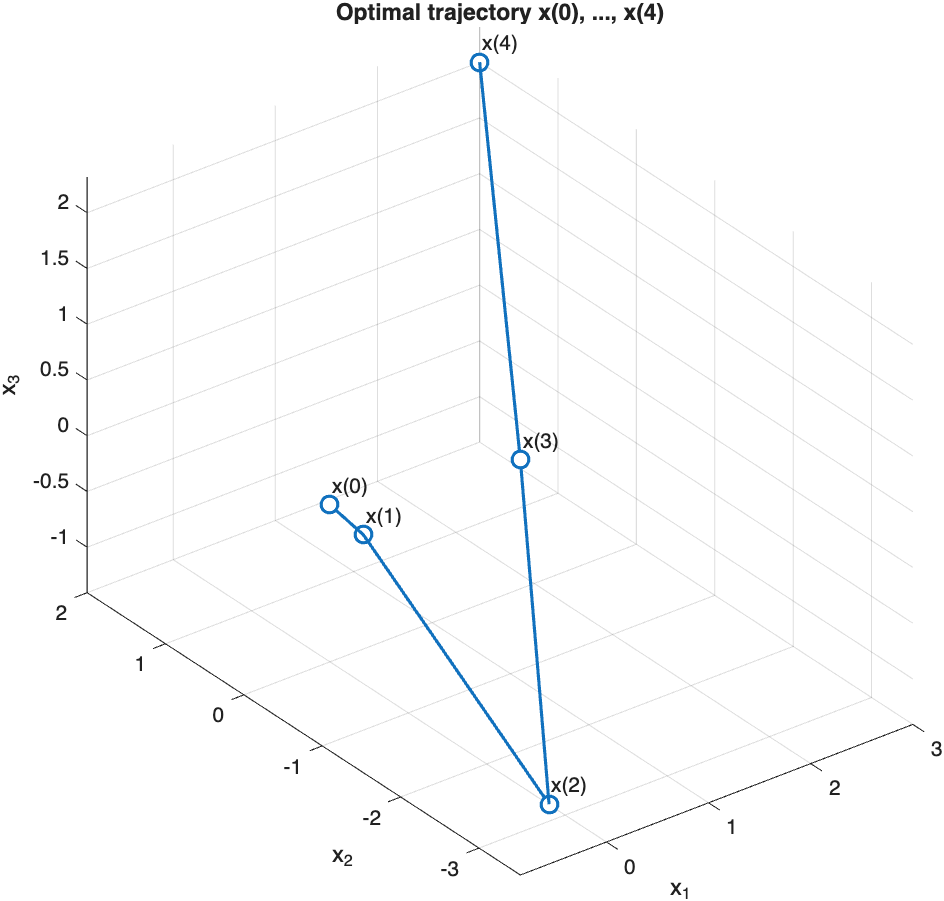
\includegraphics[width=0.7\textwidth]{problem1v.png}
                \end{figure}

            \pagebreak

            \item[vi)] Here is the optimization problem for minimizing total 
                energy with $u(0),..., u(3) \in \mathbb{R}^3$ as arguments
                \[
                    \begin{array}{rl}
                        \min\limits_{\boldsymbol{u}} & u(0)^2 + u(1)^2 + u(2)^2 + u(3)^2, \\ [2ex]
                        \text{s.t.} & x_d - H \boldsymbol{u} = 0, \\ [1ex]
                        & -3.3 \leq x_i(k) \leq 3.2, \quad i=1,2,3, \quad k=0,1,2,3,4
                    \end{array}
                \]

                where $\boldsymbol{u} = [u(0) \ u(1) \ u(2) \ u(3)]^\top$ and
                $x_d = [3 \ 2 \ 2]^\top$. I wrote a script in \texttt{problem1vi.m}
                to solve the problem numerically in CVX. The optimal sequence 
                of inputs $\boldsymbol{u}$ is $u(0) = -1.4833$, $u(1) = 
                3.1833$, $u(2) = 0.3333$, and $u(3) = -4.5333$. The minimized 
                total energy is $32.9961$. Below is a plot of the 
                optimal trajectory.

                \begin{figure}[h!]
                    \centering
                    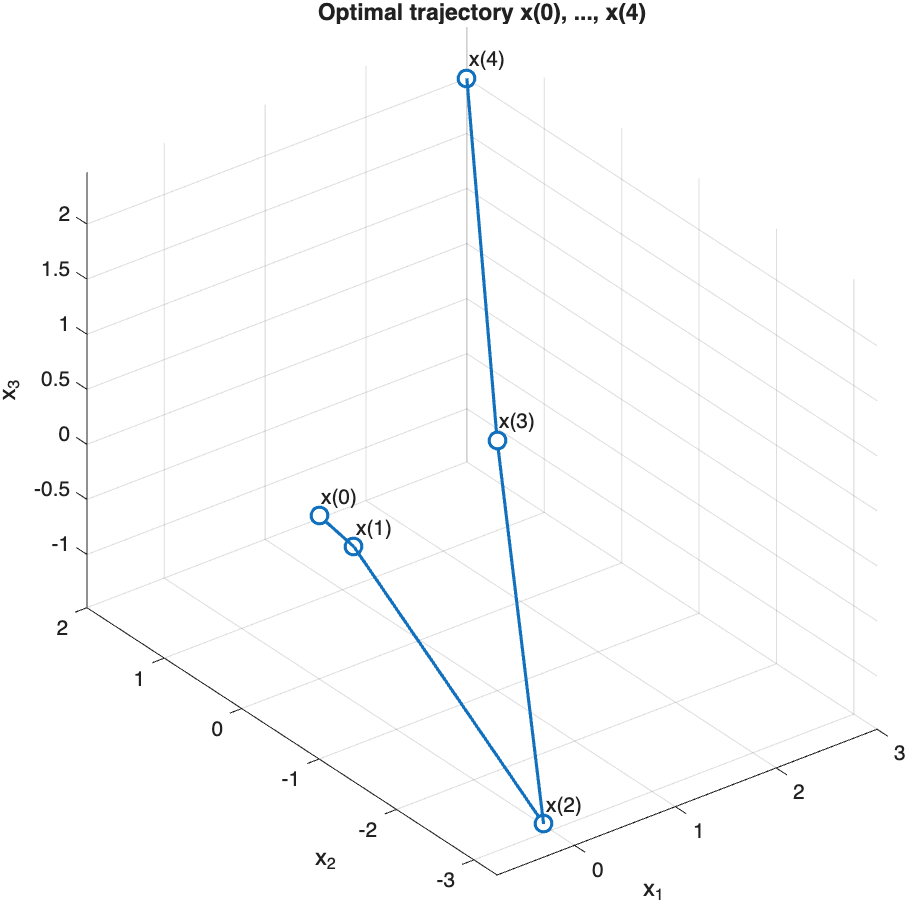
\includegraphics[width=0.7\textwidth]{problem1vi.png}
                \end{figure}

        \end{itemize}

    \end{solution}

\end{homeworkProblem}

\pagebreak

\begin{homeworkProblem}
    
    \textbf{(Coding)} Consider the matrix $A$ and vector $x^*$ defined as
    \begin{equation}
        A = \left[ \begin{array}{ccc} 
            1 & 1 & 1 \\ 
            -1& 1 & 0 \\ 
            -1& -1& 1 \\ 
            1 & 0 & 1 \\ 
            -1& 1 & 1 \\ 
            0 & -1& 1 \end{array}
            \right], \qquad 
        x^* = \left[ \begin{array}{ccc} 
            1 \\ 
            1 \\ 
            1 \end{array}
            \right]
    \end{equation}
 
    Define $b = Ax^* + v$ where $v \in \mathbb R^6$ is some measurement noise. 
    Assume that the user has no access to $x^*$ and aims to learn $x^*$ from 
    the measurement vector $b$. We consider two different estimators to learn 
    $x^*$:
    \begin{subequations}
        \begin{align}
            &\text{$l_1$ estimator:} \qquad \min_x \|Ax-b\|_1, \\
            &\text{$l_2$ estimator:} \qquad \min_x \|Ax-b\|_2
        \end{align}
    \end{subequations}

    Given a solution $\hat x$ obtained from any of the above estimators, we 
    define the estimation error $e = \|\hat x-x^*\|_2$ (note that the error 
    is always computed with respect to the $l_2$-norm no matter which estimator 
    is used for obtaining $\hat x^*$). Assume that the noise $v$ is in the form
    \begin{equation}
        v = \left[ \begin{array}{ccc}  
            t_1 \\ 
            0   \\ 
            0   \\ 
            0   \\ 
            t_2 \\ 
            0   \end{array} \right]
    \end{equation}

    where $t_1$ and $t_2$ are constants that belong to the discrete set 
    $\{-2, -1.9, -1.8, ..., -0.1, 0, 0.1, ..., 1.8, 1.9, 2\}$ (the increment 
    is $0.1$).
    
    \begin{itemize}
        \item [i)] For each possible value of the pair $(t_1, t_2)$, solve the 
            $l_1$ and $l_2$ estimators in CVX and record the corresponding 
            estimation errors (note: there are $41 \times 41$ possibilities 
            for $(t_1, t_2)$). 
        \item [ii)] Draw a grid in $\mathbb R^2$ obtained as follows: For each 
            possible value of the pair $(t_1, t_2)$, we put a symbol in the 
            location $(t_1, t_2)$ in $\mathbb R^2$, where the symbol is a small 
            red circle if the $l_1$ estimator gives the lowest estimation error 
            and is a small blue circle if the $l_2$ estimator gives the lowest 
            estimation error (note: if the estimation errors for both 
            estimators are the same, use the blue circle). Analyze the plot 
            and report your observations. 
    \end{itemize}



\end{homeworkProblem}

\pagebreak

\begin{homeworkProblem}
    
    A taxi company has $n$ taxis available and $n$ customers to be picked up as 
    soon as possible. For every $i, j \in \{1, \ldots, n\}$, if taxi $i$ decides 
    to pick up customer $j$, the amount of time (delay) to pick up the customer 
    is $d_{ij}$. Each taxi is allowed to pick up only one customer. The goal is 
    to assign each customer to a taxi so that the total delay (i.e., sum of the 
    delays for all customers) is minimized.
    \\ \\
    Formulate this assignment problem as an optimization problem.
    \\

    \begin{solution}
        \[
            \begin{array}{rl}
            \min\limits_{\boldsymbol{x}} & \underset{f_0(\boldsymbol{x})}{\boxed{\sum_{i=1}^{n} \sum_{j=1}^{n} d_{ij} x_{ij}}}, \\ [3ex]
            \text{s.t.} & \underset{f_1(\boldsymbol{x})}{\boxed{-1 + \sum_{i=1}^{n} x_{ij}}} \leq 0 \quad \forall i \in \{1, \dots, n\}, \\ [3ex]
                        & \underset{f_2(\boldsymbol{x})}{\boxed{1 - \sum_{i=1}^{n} x_{ij}}} \leq 0 \quad \forall i \in \{1, \dots, n\}, \\ [3ex]
                        & \underset{f_3(\boldsymbol{x})}{\boxed{-1 + \sum_{j=1}^{n} x_{ij}}} \leq 0 \quad \forall j \in \{1, \dots, n\}, \\ [3ex]
                        & \underset{f_4(\boldsymbol{x})}{\boxed{1 - \sum_{j=1}^{n} x_{ij}}} \leq 0 \quad \forall j \in \{1, \dots, n\}
            \end{array}
        \]
        where
        \begin{itemize}
            \item \(x_{ij} \in \{0, 1\}\) is a binary variable, where \(x_{ij} = 1\) if taxi \(i\) is assigned to customer \(j\) and \(x_{ij} = 0\) otherwise;
            \item $f_0$ : the \textit{objective function}, or \textit{total delay} for all customers;
            \item $f_1$ \& $f_2$ : the \textit{taxi assignment constraint}, each taxi can only pick up one customer;
            \item $f_3$ \& $f_4$ : the \textit{customer assignment constraint}, each customer must be picked up by exactly one taxi;
        \end{itemize}

    \end{solution}
\end{homeworkProblem}

\pagebreak

\end{document}